%*******************************************************************************
%****************************** Second Chapter *********************************
%*******************************************************************************

\chapter{The Prototype Detector}\label{Chp:ThePrototypeDetector}

\ifpdf
    \graphicspath{{Chapter2/Figs/Raster/}{Chapter2/Figs/PDF/}{Chapter2/Figs/}}
\else
    \graphicspath{{Chapter2/Figs/Vector/}{Chapter2/Figs/}}
\fi


This thesis will cover two distinct versions of the detector. The original prototype detector which was re-purposed technology from the T2K ND280 ECal \cite{Allan_2013} and an upgraded version which uses the same basic materials in the detector but upgraded electronics and containment which will be refereed to as the ``Verification Instrument for Direct Assay of Nuclear Reactors at Range'' (VIDARR) detector. The rest of this section will focus on the prototype detector.
\\\\As it is the basis for the other detectors a quick overview of the T2K ND280 ECal will be required. The ND280 is series of detectors from the neutrino oscillation experiment T2K which relies on a $\mu_nu$ beam entering the detector as show in figure \ref{fig:nd280Fig}. This detector was comprised of several different types of detector including time projection chambers (TPCs) and fine-grained detectors (FGDs) and electromagnetic calorimeters (ECals) \cite{Allan_2013}. The ECals are of particular interest as they are the basis for the prototype and VIDARR detectors. 
\begin{figure}[H]
 \centering
 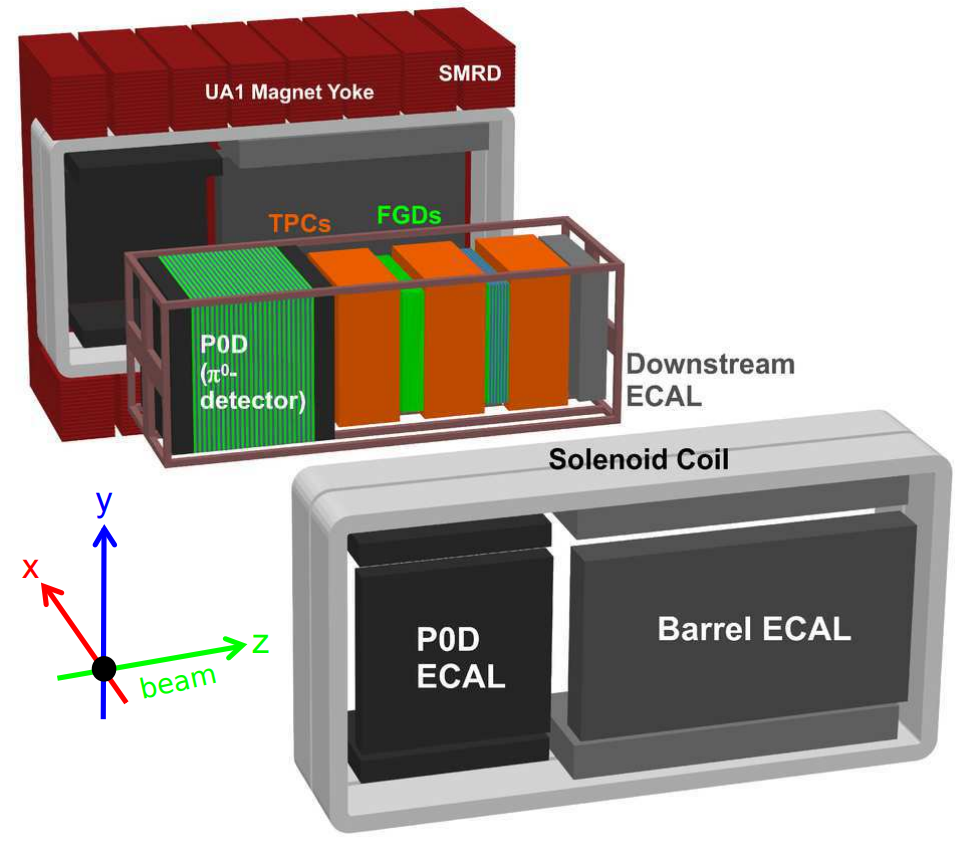
\includegraphics[width=\linewidth/2]{ND280Fig.png} 
 \captionof{figure}{Diagram of the ND280 detector. From \cite{Allan_2013}} %~can be used as a kind of place holder in latex
 \label{fig:nd280Fig}
\end{figure}
The T2K Ecals were made from plastic scintillating bars measuring 4\,cm by 1\,cm with varying lengths arranged in alternating layers at 90 degrees to each other \cite{Allan_2013}. Wavelength shifting (wls) fibres were placed in the centre of the scintillating bars which shift the wavelength from blue to green \cite{Allan_2013}. These wavelength shifting fibres are then connected to multi-pixel photon counters (MPPCs) which are the instrument which reads out the signal. This signal is then read in by Trip-T front-end electronic boards (TFBs) which then splits the signal into different cycles each containing 1.5 microseconds of information. All of this is shared by the prototype detector. 
\\\\However a crucial different between the ECals of the ND280 and the prototype detector is that the (ECals) had a layer of lead in between each of the plastic scintillating layers \cite{Allan_2013}. In the prototype this has been replaced with a layer of gadolinium so that neutrons were capture for inverse $\beta$ decay. The prototype was also designed to fit inside of a shipping container each bar having a length of 152\,cm and the whole detector measuring 152\,cm by 152\,cm with 49 layers of plastic scintillating bars totalling 49\,cm. The electronic systems were also adapted from the from the T2K system however they were altered such that they triggered on a gadolinium cascade from inverse $\beta$ decay. There were 23 cycles numbered from 0-22 with 0-17 cycles being considered "prompt" and cycle 18 is the trigger cycle. Cycles 19 -22 were left alone so that they could be compared in case time dependent issues arose from the altered system. Cycles 19-22 are useful for $\mu$ tomography as time dependent errors can arise from this adaptation of the electronics. 
\\\\The original detector was deployed at Wylfa power station in Anglesey Wales for an 18-month period. This run proved successful measuring the power on from the reactor to within good agreement to the measured reactor flux see figure \ref{fig:prototypeMeasumentFlux}. With a measured anti-neutrino rate of 172.1 $\pm$ 4.6 candidates per day when the reactor is off and 203.7 $\pm$ 19.6 when the reactor was on \cite{Carroll_2018}. Unfortunately due to cooling issues with the prototype the reactor shutdown was not observed. This is one of the main motivating factors behind the upgrade of the detector as the first generation MPPCs and reporposed electronics were susceptible to high levels of noise if the temperature was not carefully controlled. 
\begin{figure}[H]
 \centering
 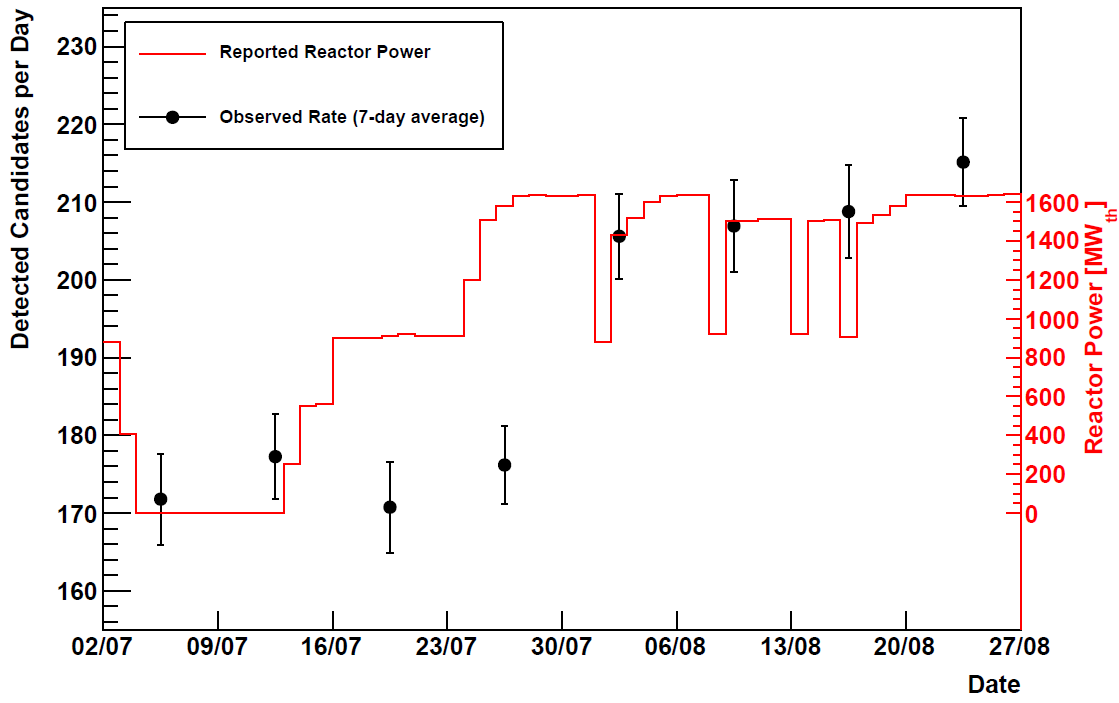
\includegraphics[width=0.90\linewidth]{prototypeMeasureOnFig.png} 
 \captionof{figure}{Measured anti-neutrino flux compared to the power generation from the Wylfa power station. From \cite{Carroll_2018}} %~can be used as a kind of place holder in latex
 \label{fig:prototypeMeasumentFlux}
\end{figure}


